\documentclass{article}

\usepackage{graphicx}
\usepackage{fancyhdr}
\usepackage[margin=1in]{geometry}
\usepackage{listings}
\usepackage[hidelinks]{hyperref}
%\usepackage{subfigure}
\usepackage{subcaption}

\usepackage{amsmath}
\usepackage{subcaption}
\usepackage{float}
\usepackage{booktabs}

\hypersetup{
	colorlinks=true,
	linkcolor=teal,
	filecolor=magenta,      
	urlcolor=teal,
	citecolor = teal
}
\usepackage{xcolor}
\usepackage{xepersian}
\setlength\headheight{28pt} 
\settextfont[
    Path = ./font/, % specify the path to the font files
    Scale = 1.3,
    UprightFont = XB Niloofar, % Regular font
    BoldFont = XB NiloofarBd,       % Bold font
    ItalicFont = XB NiloofarIt,   % Italic font
    BoldItalicFont = XB NiloofarBdIt % Bold Italic font if available
]{XB Niloofar}
\setlatintextfont[Scale=1.3]{Times New Roman}
\renewcommand{\baselinestretch}{1.5}
\pagestyle{fancy}
\fancyhf{}
\rhead{
\includegraphics[width=1cm]{img/Logo.png} 
	یادگیری ماشین
	-
	مینی پروژه شماره 2}
\lhead{\thepage}
\rfoot{سیدمحمد حسینی}
\lfoot{9821253}
\renewcommand{\headrulewidth}{1pt}
\renewcommand{\footrulewidth}{1pt}
\renewcommand{\lstlistingname}{Code}

\definecolor{codegreen}{rgb}{0,0.6,0}
\definecolor{codegray}{rgb}{0.5,0.5,0.5}
\definecolor{codepurple}{rgb}{0.58,0,0.82}
\definecolor{backcolour}{rgb}{0.95,0.95,0.92}

\lstdefinestyle{mystyle}{
	backgroundcolor=\color{backcolour},   
	commentstyle=\color{codegreen},
	keywordstyle=\color{magenta},
	numberstyle=\tiny\color{codegray},
	stringstyle=\color{codepurple},
	basicstyle=\ttfamily\footnotesize,
	breakatwhitespace=false,         
	breaklines=true,                 
	captionpos=b,                    
	keepspaces=true,                 
	numbers=left,                    
	numbersep=5pt,                  
	showspaces=false,                
	showstringspaces=false,
	showtabs=false,                  
	tabsize=2
}

\lstset{style=mystyle}

\begin{document}
	
	\begin{titlepage}
\begin{center}
\defpersianfont\nast[Path={./font/}, Scale=2]{IranNastaliq}
\centerline{{
\includegraphics[width=5cm]{img/Logo.png}}}
\centerline{\textcolor[rgb]{0,0,0.5}{\nast \large  دانشگاه صنعتی خواجه نصیرالدین طوسی}}
\centerline{\textcolor[rgb]{0,0,0.5}{\nast \bfseries دانشکدۀ مهندسی برق - گروه مهندسی کنترل}}

\vfill
        
\Huge
\textbf{یادگیری ماشین}\\
\textbf{پاسخ مینی پروژه دوم}\\
        
\vfill
\large
    نام و نام خانوادگی:  سیدمحمد حسینی\\
    شمارۀ دانشجویی: 9901399\\
    تاریخ: مهرماه 1402\\

\href{https://github.com/mamdaliof/MachineLearning2024W}{GitHub}

\href{https://drive.google.com/drive/folders/10-8uiqpIUbC2HcEtwjqP1IAix46nCrbL?usp=sharing}{Google Drive}


\end{center}
\end{titlepage}

	
	\tableofcontents \clearpage
	\listoffigures \clearpage
	\listoftables \clearpage
	\lstlistoflistings \clearpage
	\newpage
	
\section{سوال 2}

\subsection{مشکل مورد بررسی}

مقاله به چالش مدل‌های مبتنی بر SVM به منظور طبقه‌بندی چندکلاسه می‌پردازد. SVMهای سنتی ، عملکرد
 \lr{Binary Classification }
 دارند این در حالی که برای مسائل چند کلاسه، نیاز به سازگار کردن مدل یا رویکرد تصمیم‌گیری، به منظور مدیریت تمام کلاس‌ها می‌باشد. رویکردهای کلاسیک موجود مانند روش‌های 
 \lr{one-vs-one}‎
  و
  \lr{one-vs-all}
  ، اگرچه محبوب هستند، محدودیت‌هایی دارند. روش
  \lr{one-vs-one}
   شامل حل
 $K(K-1)$ 
 مسئله دودویی است که برای
 $K$های
 بزرگ باعث افزایش شدید بار محاسباتی می‌شود. از سوی دیگر، روش
 \lr{one-vs-all}
  می‌تواند مناطق تصمیم‌گیری ایجاد کند که متعلق به هیچ کلاسی نمی‌باشد.

\subsection{روش پیشنهادی}

در این مقاله یک مدل به اسم
\lr{Generalized Multiclass Support Vector Machine (GenSVM) }
پیشنهاد داده شده است که برای مدیریت طبقه‌بندی چندکلاسه بدون تجزیه مسئله به چندین طبقه‌بندی دودویی طراحی شده است. روش GenSVM از بهینه‌سازی 
\lr{iterative majorization}
، یک تکنیک بهینه‌سازی ریاضی، برای حل مسئله طبقه‌بندی استفاده می‌کند. این روش یک تابع بزرگی ایجاد می‌کند که به حداقل رساندن آن آسان‌تر از تابع هدف اصلی است و تضمین می‌کند که به سمت راه‌حل بهینه همگرا می‌شود. الگوریتم بهینه‌سازی تکراری شامل مراحل تعیین نقطه شروع، به حداقل رساندن تابع بزرگی و تکرار تا همگرایی است. دلیل استفاده از این الگوریتم این است که عموما بهینه کردن یک تابع dual می‌تواند هزینه محاسباتی زیادی داشته باشد.

\subsection{ارزیابی عملکرد}

عملکرد GenSVM با استفاده از آزمایشات گسترده‌ای محاسبه شده است تا با بقیه مدل‌های موجود در زمینه SVMهای چندکلاسه مقایسه شود. برای ارزیابی جامع عملکرد، از مجموعه داده‌های بزرگ و کوچک استفاده شد. استفاده از مجموعه داده‌های بزرگ به منظور بررسی مقیاس‌پذیری و کارایی محاسباتی در شرایط واقعی بود، در حالی که مجموعه داده‌های کوچک به منظور بررسی دقت طبقه‌بندی و قابلیت تعمیم در شرایط مختلف مورد استفاده قرار گرفتند.

برای مقایسه روش‌ها، از شاخص 
 \lr{adjusted Rand index (ARI) }
 برای اندازه‌گیری دقت طبقه‌بندی و همچنین از روش‌های رتبه‌بندی برای ارزیابی کارایی نسبی استفاده شد. روش رتبه‌بندی بر اساس زمان آموزش و دقت طبقه‌بندی هر روش انجام شد. در این مطالعه، GenSVM با چندین روش موجود در زمینه SVMهای چندکلاسه مقایسه شد که شامل روش‌های
 \lr{one-vs-one، one-vs-all}
  و سایر روش‌های بهینه‌سازی چندکلاسه می‌شود.

نتایج نشان داد که GenSVM به طور قابل توجهی از نظر دقت طبقه‌بندی و کارایی محاسباتی برتری دارد. GenSVM بهترین نتایج را برای سریع‌ترین روش در جستجوی شبکه‌ای داشت و زمان آموزش متوسط آن به طور قابل توجهی کمتر از سایر روش‌ها بود. علاوه بر این، این روش نشان داد که در مقابل داده‌های مختلف مقاوم و قابل توسعه است و مقیاس‌پذیری و قابلیت اطمینان آن را نشان می‌دهد. این مدل بعد از روش
\lr{one-vs-one}
 بهترین دقت را کسب کرده است.

\subsection{مزایا و معایب}

\textbf{مزایا:}
\begin{itemize}
    \item \textbf{سرعت}: GenSVM زمان محاسبات را به طور قابل توجهی نسبت به روش‌های سنتی کاهش می‌دهد.
    \item \textbf{دقت}: این روش از نظر دقت طبقه‌بندی از اکثر روش‌های موجود پیشی می‌گیرد.
    \item \textbf{مقیاس‌پذیری}: GenSVM مقاوم و مقیاس‌پذیر است و در مقابل مجموعه داده‌های مختلف عملکرد خوبی دارد.
    \item \textbf{حذف ناحیه ابهام}: خروجی این مدل، فضای ویژگی‌ها را به گونه‌ای افراز می‌کند که هیچ ناحیه‌ای بدون کلاس مشخص وجود نداشته باشد.
    \item \textbf{یک مدل به عنوان خروجی}: در این مدل به جای آموزش چندین svm برای تشخیص هر کلاس، یک مدل آموزش داده می‌شود که تمامی کلاس‌ها را پیشبینی کند.
\end{itemize}

\textbf{معایب:}
\begin{itemize}
    \item \textbf{پیچیدگی}: پیاده‌سازی بهینه‌سازی تکراری و مدیریت مجموعه‌ای بزرگتر از hyperparameterها
     می‌تواند پیچیده باشد .
    \item \textbf{منابع مورد نیاز}: علیرغم بهبودهای کارایی، نیاز اولیه به منابع محاسباتی می‌تواند بالا باشد، به ویژه برای مجموعه داده‌های بسیار بزرگ درحالی که بخواهیم تمام 
    hyperparameterهای 
    موجود را بررسی کنیم.
\end{itemize}

در نتیجه، روش پیشنهادی GenSVM پیشرفت قابل توجهی در زمینه طبقه‌بندی چندکلاسه با SVMها ارائه می‌دهد، دقت و کارایی بهتری را به ارمغان می‌آورد، اگرچه با افزایش پیچیدگی و نیازهای منابع همراه است.





\subsection{مشکل مورد بررسی}

مقاله به چالش مدل‌های مبتنی بر SVM به منظور طبقه‌بندی چندکلاسه می‌پردازد.
\lr{ SVM}های سنتی، عملکرد
\lr{Binary Classification}
دارند این در حالی که برای مسائل چند کلاسه، نیاز به سازگار کردن مدل یا رویکرد تصمیم‌گیری، به منظور مدیریت تمام کلاس‌ها می‌باشد. 

به صورت کلی سه نوع رویکرد برای SVMهای چندکلاسه وجود دارد: روش‌های 
heuristic
که شامل 
\lr{one-vs-one}‎
 و 
 \lr{one-vs-all}
  می‌باشد.
روش‌های مذکور 
\lr{one-vs-one}‎
و
\lr{one-vs-all}،
اگرچه محبوب و پر استفاده هستند، محدودیت‌هایی دارند. روش
\lr{one-vs-one}
شامل حل
$K(K-1)$ 
مسئله دودویی است که برای
$K$های
بزرگ باعث افزایش شدید بار محاسباتی می‌شود. از سوی دیگر، روش
\lr{one-vs-all}
باید k مرتبه تمام دیتاست را استفاده کند تا یک مدل طبقه‌بندی ایجاد کند . این روش‌ها که مبتنی بر تبدیل مسئله به زیرمسئله‌های کوچکتر است، می‌تواند مناطق تصمیم‌گیری ایجاد کنند که متعلق به هیچ کلاسی نمی‌باشد.

روش دیگر مبتنی بر اصلاح خطا می‌باشد که حالت کلی‌تر روش قبلی می‌باشد. ایراد مدل‌های مبتنی بر این روش این است که ماتریس اصلاح باید از قبل مشخص باشد که در بسیاری از موارد انجام اینکار بسیار دشوار است. آخرین روش مبتنی بر طراحی و آموزش مدل‌هایی است که مستقیما مسئله چند کلاسه را با استفاده از یک ماشین SVM حل کند.

\subsection{روش پیشنهادی}

در این مقاله یک مدل به اسم
\lr{Generalized Multiclass Support Vector Machine (GenSVM)}
پیشنهاد داده شده است که برای مدیریت طبقه‌بندی چندکلاسه بدون تجزیه مسئله به چندین طبقه‌بندی دودویی طراحی شده است. روش GenSVM از بهینه‌سازی
\lr{iterative majorization}،
یک تکنیک بهینه‌سازی ریاضی، برای حل مسئله طبقه‌بندی استفاده می‌کند. این روش یک تابع بزرگی ایجاد می‌کند که به حداقل رساندن آن آسان‌تر از تابع هدف اصلی است و تضمین می‌کند که به سمت راه‌حل بهینه همگرا می‌شود. الگوریتم بهینه‌سازی تکراری شامل مراحل تعیین نقطه شروع، به حداقل رساندن تابع بزرگی و تکرار تا همگرایی است. دلیل استفاده از این الگوریتم این است که عموماً بهینه کردن یک تابع دوگان می‌تواند هزینه محاسباتی زیادی داشته باشد.

GenSVM یک طبقه‌بند تک‌ماشینه است که از فضای 
Simplex
 استفاده می‌کند. 
 Simplex
  فضایی است که در آن بردارهای ویژگی‌ها به نقاطی در داخل یک مثلث نگاشت می‌شوند. یکی از مزایای استفاده از فضای 
  Simplex
   این است که تصمیم‌گیری در این فضا ساده‌تر است و مرزهای تصمیم‌گیری به طور طبیعی شکل می‌گیرند. 

این مدل از تابع هزینه
\lr{Huber Hinge}
استفاده می‌کند که مشتق‌پذیر می‌باشد. نگاشت از فضای ورودی به فضای 
Simplex
 با کمینه‌سازی خطاهای طبقه‌بندی بهینه‌سازی می‌شود که با اندازه‌گیری فاصله یک نمونه از مرزهای تصمیم‌گیری در فضای 
 Simplex
  محاسبه می‌شود. پیش‌بینی کلاس نیز در همین فضای 
  Simplex
   انجام می‌شود.

در بهینه‌سازی تابع هزینه این مدل 
$p$-نرم
را بهینه می‌کند. مرزهای تصمیم‌گیری این مدل در فضای 
Simplex
 به مثلثی مربوط می‌شوند که نقاط درون آن به کلاس‌های مختلف تعلق دارند. تابع زیان GenSVM این امکان را فراهم می‌کند که مدل‌های تک‌ماشینه قبلی در قالب طبقه‌بندهای نوع سوم پیاده‌سازی شوند.

\subsection{ارزیابی عملکرد}

عملکرد GenSVM با استفاده از آزمایشات گسترده‌ای محاسبه شده است تا با بقیه مدل‌های موجود در زمینه SVMهای چندکلاسه مقایسه شود. برای ارزیابی جامع عملکرد، از مجموعه داده‌های بزرگ و کوچک استفاده شد. استفاده از مجموعه داده‌های بزرگ به منظور بررسی مقیاس‌پذیری و کارایی محاسباتی در شرایط واقعی بود، در حالی که مجموعه داده‌های کوچک به منظور بررسی دقت طبقه‌بندی و قابلیت تعمیم در شرایط مختلف مورد استفاده قرار گرفتند.

برای مقایسه روش‌ها، از شاخص
\lr{adjusted Rand index (ARI)}
برای اندازه‌گیری دقت طبقه‌بندی و همچنین از روش‌های رتبه‌بندی برای ارزیابی کارایی نسبی استفاده شد. روش رتبه‌بندی بر اساس زمان آموزش و دقت طبقه‌بندی هر روش انجام شد. در این مطالعه، GenSVM با چندین روش موجود در زمینه SVMهای چندکلاسه مقایسه شد که شامل روش‌های
\lr{one-vs-one، one-vs-all}
و سایر روش‌های بهینه‌سازی چندکلاسه می‌شود.

نتایج نشان داد که GenSVM به طور قابل توجهی از نظر دقت طبقه‌بندی و کارایی محاسباتی برتری دارد. GenSVM بهترین نتایج را برای سریع‌ترین روش در جستجوی شبکه‌ای داشت و زمان آموزش متوسط آن به طور قابل توجهی کمتر از سایر روش‌ها بود. علاوه بر این، این روش نشان داد که در مقابل داده‌های مختلف مقاوم و قابل توسعه است و مقیاس‌پذیری و قابلیت اطمینان آن را نشان می‌دهد. این مدل بعد از روش
\lr{one-vs-one}
بهترین دقت را کسب کرده است.

\subsection{مزایا و معایب}

\textbf{مزایا:}
\begin{itemize}
    \item \textbf{سرعت}: GenSVM زمان محاسبات را به طور قابل توجهی نسبت به روش‌های سنتی کاهش می‌دهد.
    \item \textbf{دقت}: این روش از نظر دقت طبقه‌بندی از اکثر روش‌های موجود پیشی می‌گیرد.
    \item \textbf{مقیاس‌پذیری}: GenSVM مقاوم و مقیاس‌پذیر است و در مقابل مجموعه داده‌های مختلف عملکرد خوبی دارد.
    \item \textbf{حذف ناحیه ابهام}: خروجی این مدل، فضای ویژگی‌ها را به گونه‌ای افراز می‌کند که هیچ ناحیه‌ای بدون کلاس مشخص وجود نداشته باشد.
    \item \textbf{یک مدل به عنوان خروجی}: در این مدل به جای آموزش چندین SVM برای تشخیص هر کلاس، یک مدل آموزش داده می‌شود که تمامی کلاس‌ها را پیش‌بینی کند.
\end{itemize}

\textbf{معایب:}
\begin{itemize}
    \item \textbf{پیچیدگی}: پیاده‌سازی بهینه‌سازی تکراری و مدیریت مجموعه‌ای بزرگتر از hyperparameterها می‌تواند پیچیده باشد.
    \item \textbf{منابع مورد نیاز}: علیرغم بهبودهای کارایی، نیاز اولیه به منابع محاسباتی می‌تواند بالا باشد، به ویژه برای مجموعه داده‌های بسیار بزرگ درحالی که بخواهیم تمام hyperparameterهای موجود را بررسی کنیم.
\end{itemize}

در نتیجه، روش پیشنهادی GenSVM پیشرفت قابل توجهی در زمینه طبقه‌بندی چندکلاسه با SVMها ارائه می‌دهد، دقت و کارایی بهتری را به ارمغان می‌آورد، اگرچه با افزایش پیچیدگی و نیازهای منابع همراه است.

\section{سوال 3}

در ادامه حل این سوال مجموعه داده دارو درنظر گرفته شده است و الگوریتم‌ها به روی این مجموعه داده اجرا شده‌اند.
در ادامه تحلیل آماری مجموعه داده دارو انجام شده است. همانطور که در 
\autoref{fig:Q3 stat}
مشخص شده است این دیتاست تا حدی 
imbalance
است و فراوانی داروی x و y بیشتر از باقی داروها می‌باشد اعداد دقیق مربوط به فراوانی این دیتاست در ‎
\autoref{Q3 stat}
نشان‌داده‌شده است.
\begin{figure}[H]
\centering
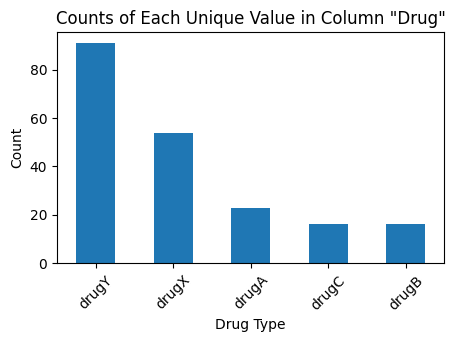
\includegraphics[width=1\linewidth]{img/Q3/stat}
\caption{نمودار توزیع داده}
\label{fig:Q3 stat}
\end{figure}

\begin{LTR}
\label{Q3 stat}
\begin{verbatim}
The number of unique values in the column "Drug" is 5
drugY    91
drugX    54
drugA    23
drugC    16
drugB    16
Name: Drug, dtype: int64

\end{verbatim}
\end{LTR}

\autoref{tab:Q3 Table}
نشان‌دهنده چند سطر از مجموعه داده دارو می‌باشد که مقادیر توصیفی ستون‌های 
Sex، BP و Cholesterol 
به شرح زیر می‌باشد:
\begin{LTR}
\label{Q3 stat}
\begin{verbatim}
Values of Sex column =  ['F' 'M']
Values of BP column =  ['HIGH' 'LOW' 'NORMAL']
Values of Cholesterol column ['HIGH' 'NORMAL']
\end{verbatim}
\end{LTR}


\begin{table}[H]
\centering
\begin{tabular}{ccccccc}
\toprule
 & Age & Sex & BP & Cholesterol & Na\_to\_K & Drug \\
\midrule
0 & 23 & F & HIGH & HIGH & 25.355 & drugY \\
1 & 47 & M & LOW & HIGH & 13.093 & drugC \\
2 & 47 & M & LOW & HIGH & 10.114 & drugC \\
3 & 28 & F & NORMAL & HIGH & 7.798 & drugX \\
4 & 61 & F & LOW & HIGH & 18.043 & drugY \\
\bottomrule
\end{tabular}
\caption{Sample Data}
\label{tab:Q3 Table}
\end{table}

\subsection{بخش اول}



{\large \textbf{سوال}:} 

توضیح دهید که از چه روشی برای انتخاب بخشی از داده استفاده کرده‌اید. آیا روش بهتری برای این کار می‌شناسید؟



{\large \textbf{سوال}:} 

به منظور پاسخ داده به این سوال ابتدا باید کدی که به وسیله آن دیتاست تقسیم شده است مورد بررسی قرار بگیرد.
کد زیر به منظور تقسیم دیتاست موجود به دو زیرمجموعه آموزش و ارزیابی است که در نتیجه آن
40\% 
 از این دیتاست با توزیع یکنواخت به مجموعه ارزیابی تخصیص داده می‌شود.

\begin{LTR}
	\begin{lstlisting}[language=Python, caption=Data Selection]
		X_train, X_test, y_train, y_test = train_test_split(X, y, test_size=0.4, random_state=53)
	\end{lstlisting}
\end{LTR}

نکته حائز اهمیت این است که این دیتاست از تفکیک پذیری بالایی برخوردار است و نیازی نیست که از روش‌های پیشرفته‌تر به منظور تقسیم آن استفاده کنیم اما با توجه به 
imbalance
بودن این دیتاست می‌توان از روش 
stratify
به منظور حفظ توزیع داده‌ها و یا روش
K-Fold-cross-validation
استفاده کرد تا بهترین نتیجه ممکن را بدست آورد و از عملکرد مدل مطمئن شد.

در ادامه با استفاده از کد زیر و 
Configuration
پیش‌فرض کتابخانه
sklearn
یک درخت تصمیم ایجاد شده است و روی دیتاست آموزش، آموزش دیده است. نتایج بدست آمده از این آموزش در 
\autoref{fig Q3 :basic-tree}
نشان داده شده است.
\begin{LTR}
	\begin{lstlisting}[language=Python, caption=Train Decision Tree]
# Create a Decision Tree Classifier
clf = DecisionTreeClassifier(random_state=53)

# Train the classifier on the training data
clf.fit(X_train, y_train)

plot_tree(clf, filled=True, feature_names=X.columns, class_names=clf.classes_, rounded=True)
plt.title('Decision Tree')
plt.show()
	\end{lstlisting}
\end{LTR}


\begin{figure}[H]
\centering
\includegraphics[width=1\linewidth]{"img/Q3/basic tree"}
\caption{}
\label{fig Q3 :basic-tree}
\end{figure}

\subsection{بخش دوم}
با توجه به 
‎\autoref{fig Q3 :basic-tree}
 می‌توان مشخص کرد که از داده‌های جنسیت به منظور تعیین کلاس هر نمونه استفاده نشده است. به منظور تحلیل این مسئله لازم است تا پراکندگی جنسیت، نسبت به هر نوع دارو رسم شود. این نمودار در 
\autoref{fig:drug-vs-sex}
 رسم شده و است و همانطور که مشخص است میزان مردان نسبت به زنان همواره از 
 entropy
 بالایی برخوردار بوده که به همین دلیل نیز جنسیت در نوع دارو تاثیر چندانی نگذاشته است، به بیان دیگر این بیماری با جنسیت وابستگی پایینی دارد.
 
 
\begin{figure}[H]
\centering
\includegraphics[width=0.5\linewidth]{"img/Q3/drug vs sex"}
\caption{Sex over Drug}
\label{fig:drug-vs-sex}
\end{figure}

در ادامه متریک‌‌های موردنیاز به منظور بررسی نتایج مدل محاسبه شده است. همانطور که مشخص است برای دو زیرمجموعه آموزش و ارزیابی تمامی متریک‌های و ماتریس درهم‌ریختگی در 
\autoref{fig: Q3 basic cm}
مقداری برابر 1 دارند که این به معنی عملکرد بی‌عیب مدل ما است.
\begin{LTR}
\begin{verbatim}
training metrics:
Classification Report:
               precision    recall  f1-score   support

       drugA       1.00      1.00      1.00        17
       drugB       1.00      1.00      1.00        11
       drugC       1.00      1.00      1.00        11
       drugX       1.00      1.00      1.00        38
       drugY       1.00      1.00      1.00        63

    accuracy                           1.00       140
   macro avg       1.00      1.00      1.00       140
weighted avg       1.00      1.00      1.00       140

test metrics:

Classification Report:
               precision    recall  f1-score   support

       drugA       1.00      1.00      1.00         6
       drugB       1.00      1.00      1.00         5
       drugC       1.00      1.00      1.00         5
       drugX       1.00      1.00      1.00        16
       drugY       1.00      1.00      1.00        28

    accuracy                           1.00        60
   macro avg       1.00      1.00      1.00        60
weighted avg       1.00      1.00      1.00        60
\end{verbatim}
\end{LTR}

\begin{figure}[H] 
	\centering
	\subfigure[]{
		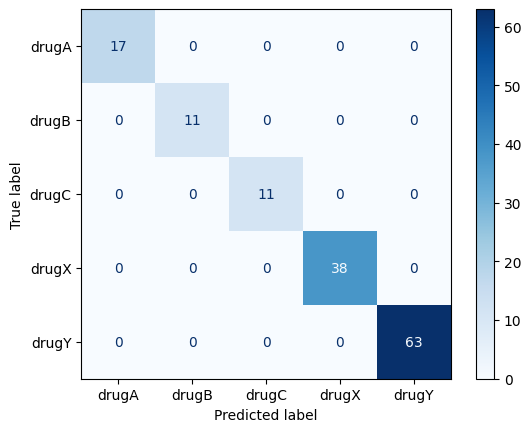
\includegraphics[width=0.4\linewidth]{img/Q3/Basic train.png}
		}
	\subfigure[]{
		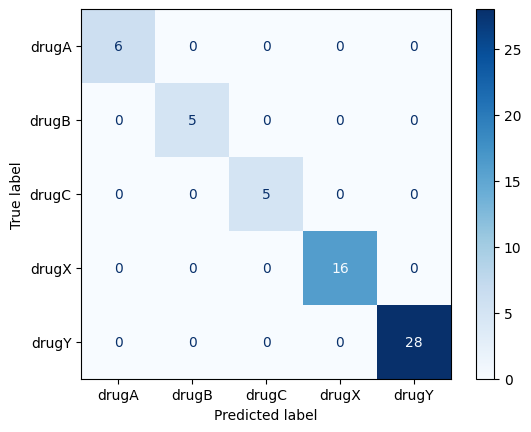
\includegraphics[width=0.4\linewidth]{img/Q3/Basic test.png}
		}
	\caption{Confusion Matrix}
	\label{fig: Q3 basic cm}
\end{figure}

حال با استفاده از 
\texttt{GridSearchCV}
هایپرپارامتر‌های متفاوت را با استفاده از متد
5-fold-corss-validation
بررسی می‌کنیم تا بهترین ساختار مدل را پیدا کنیم. در این جستجو مقادیر
\texttt{max\_depth}، \texttt{min\_samples\_split} و \texttt{min\_samples\_leaf}
را در یک بازه متناسب با دیتاستی که در اختیار داریم تغییر می‌دهیم. کد زیر به منظور آموزش مدل‌های مختلف استفاده شده است و در انتها بهترین هایپرپارامترها را خروجی می‌دهد.
\begin{LTR}
	\begin{lstlisting}[language=Python, caption=Grid search]
param_grid = {
    'max_depth': [2, 3, 4, 5, 10, 15 ],
    'min_samples_split':  [2, 5, 10, 15],
    'min_samples_leaf': [1, 2, 4, 7, 10]
}
scoring = {
    'precision': make_scorer(precision_score, average='macro'),
    'recall': make_scorer(recall_score, average='macro')
}
# Perform grid search with cross-validation
grid_search = GridSearchCV(estimator=clf, param_grid=param_grid,
                           scoring=scoring, refit='precision', return_train_score=True)
grid_search.fit(X_train, y_train)
	\end{lstlisting}
\end{LTR}

نتایج بدست آمده از این گروه آموزش‌ها نشان می‌دهد که مدل بهینه هایپرپارامتر‌های زیر را دارد.

\begin{LTR}
\begin{verbatim}
Best Parameters: {'max_depth': 4, 'min_samples_leaf': 1, 'min_samples_split': 2}
\end{verbatim}
\end{LTR}

نمودارهای موجود در 
\autoref{fig:Q3 hyper}
به ازای تغییرات هر هایپرپارامتر کشیده شده است. همانطور که مشخص است، متغییر 
\texttt{min\_samples\_split}
با افزایش مقدار، گاهی موجب بهبود و گاهی موجب افت عملکرد مدل می‌شود که این بهبود یا افت به مقدار دو متغییر دیگر بستگی دارد بنابراین نمیتوان به صورت کلی نظر قطعی درمورد این متغییر داد.
متغییر 
\texttt{max\_depth}
یک رفتار تکرار شونده را نشان می‌دهد که به غیر از مقادیر خاص، نمودار آن افزایشی می‌باشد بنابراین افزایش مقدار این متغییر می‌تواند به بهبود مدل کمک کند.
در انتها متغییر
\texttt{min\_samples\_leaf}
و نمودار مربوط به آن نشان می‌دهد که با افزایش مقدار این متغییر عملکرد مدل در این مسئله به خصوص کاهش پیدا می‌کند بنابراین کمترین مقدار ممکن را برای این متغییر درنظر می‌گیریم. 

\begin{figure}[H]
\centering
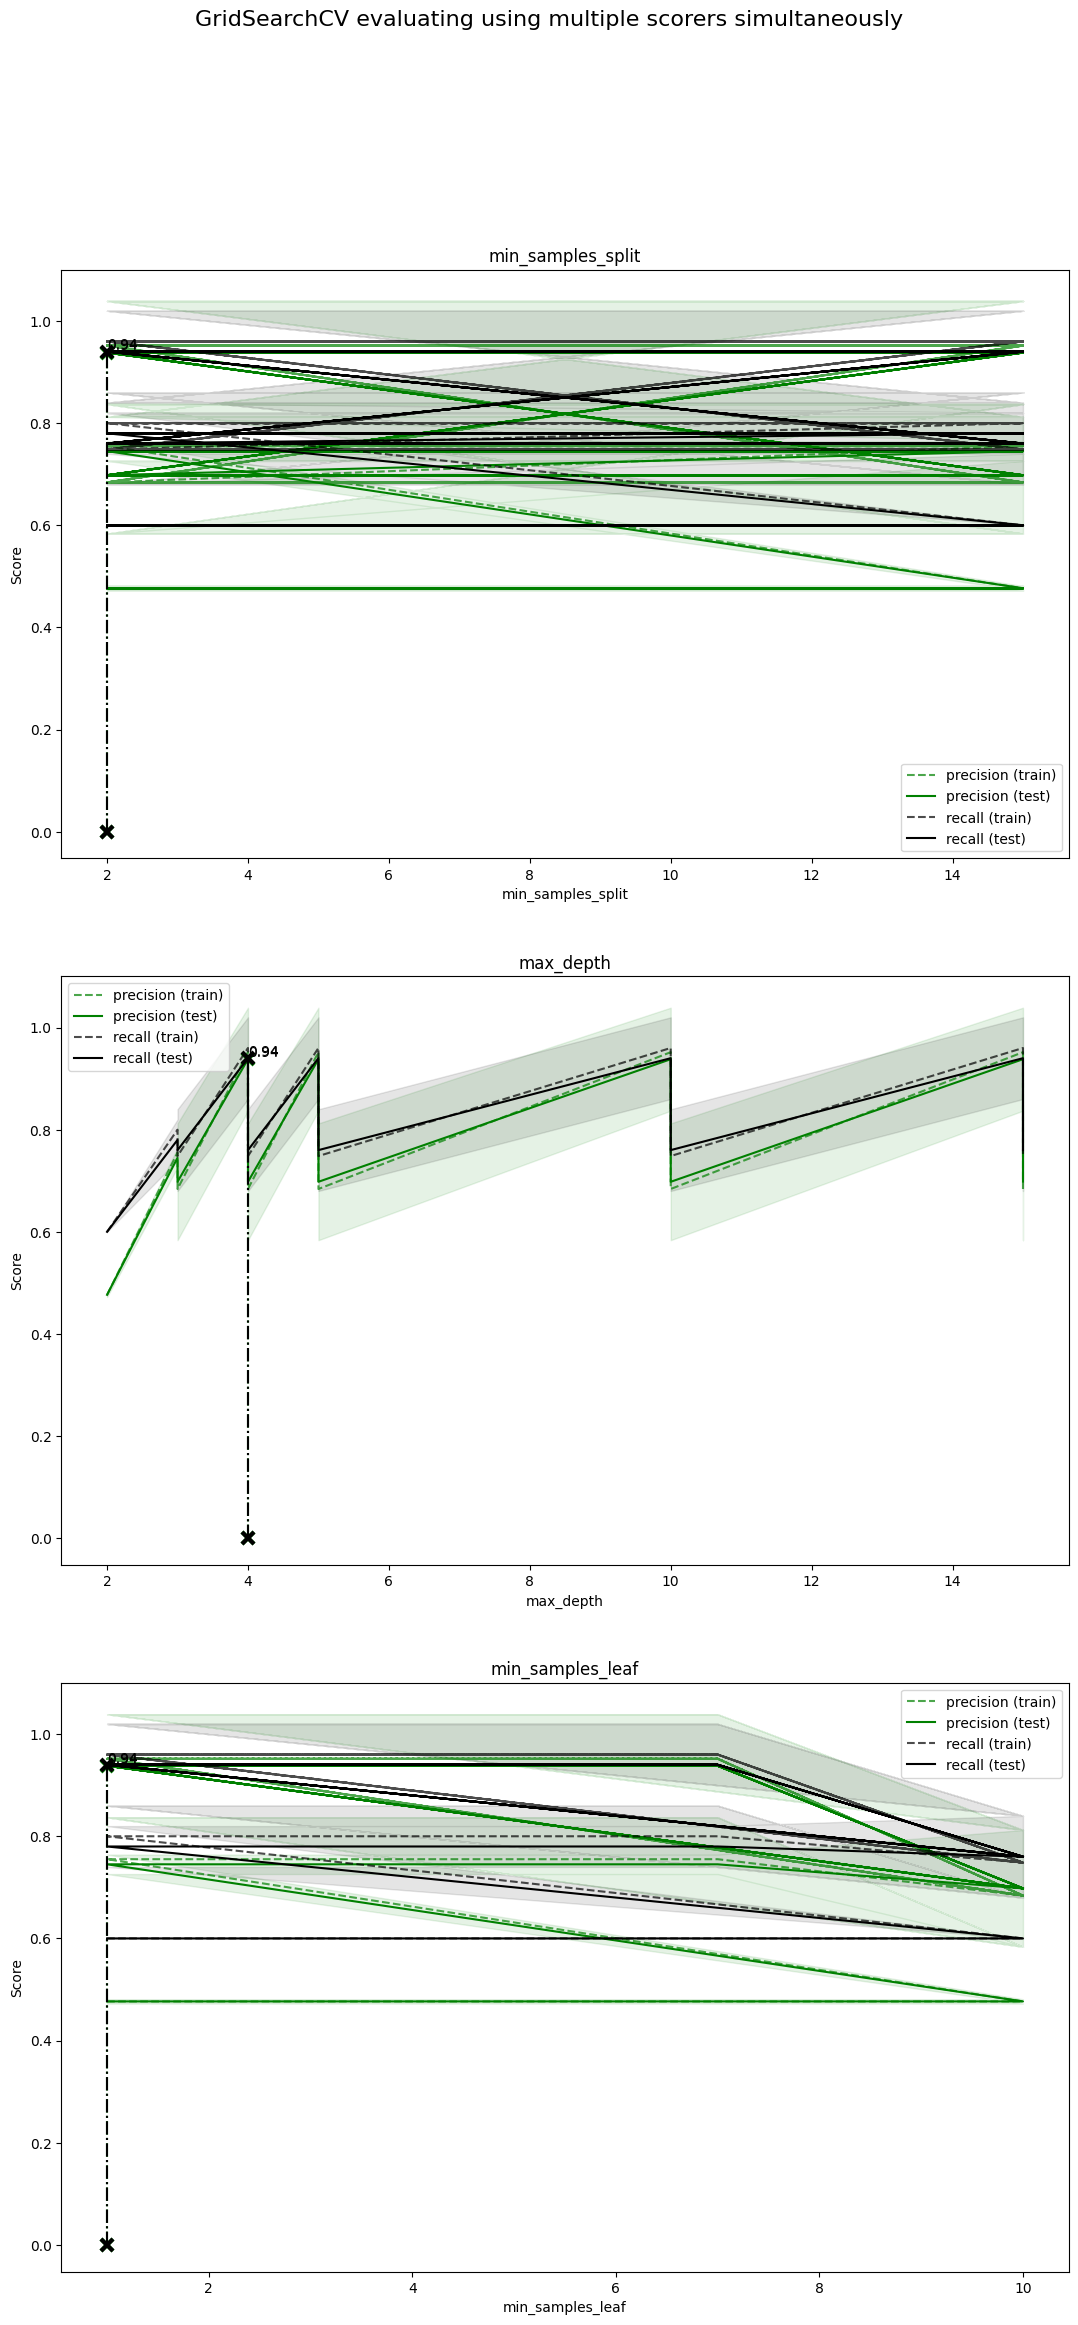
\includegraphics[height=0.9\textheight]{img/Q3/hyper}
\caption{Hyper-parameters Graph}
\label{fig:Q3 hyper}
\end{figure}

حال به سراغ بررسی نتایج بدست آمده از بهترین مدل می‌رویم، همانطور که در 
\autoref{fig:best-tree}
مشخص است، تفاوتی با درخت موجود در 
\autoref{fig Q3 :basic-tree}
نداشته است، از طرف دیگر با توجه به متریک‌ها و ماتریس درهم‌ریختگی در 
\autoref{fig: Q3 best cm}
همچنان عملکرد مدل در بهترین حالت خود می‌باشد و تمام نمونه‌ها را به درستی تشخیص داده است
\begin{figure}[H]
\centering
\includegraphics[width=0.7\linewidth]{"img/Q3/Best tree"}
\caption{Best Tree}
\label{fig:best-tree}
\end{figure}

\begin{LTR}
\begin{verbatim}
training metrics:
Classification Report:
               precision    recall  f1-score   support

       drugA       1.00      1.00      1.00        17
       drugB       1.00      1.00      1.00        11
       drugC       1.00      1.00      1.00        11
       drugX       1.00      1.00      1.00        38
       drugY       1.00      1.00      1.00        63

    accuracy                           1.00       140
   macro avg       1.00      1.00      1.00       140
weighted avg       1.00      1.00      1.00       140

test metrics:

Classification Report:
               precision    recall  f1-score   support

       drugA       1.00      1.00      1.00         6
       drugB       1.00      1.00      1.00         5
       drugC       1.00      1.00      1.00         5
       drugX       1.00      1.00      1.00        16
       drugY       1.00      1.00      1.00        28

    accuracy                           1.00        60
   macro avg       1.00      1.00      1.00        60
weighted avg       1.00      1.00      1.00        60
\end{verbatim}
\end{LTR}

\begin{figure}[H] 
	\centering
	\subfigure[]{
		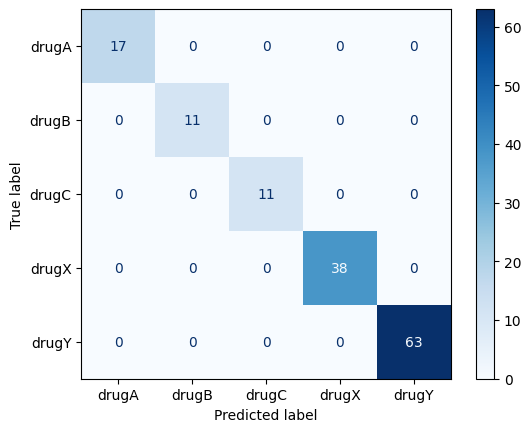
\includegraphics[width=0.4\linewidth]{img/Q3/Basic train.png}
		}
	\subfigure[]{
		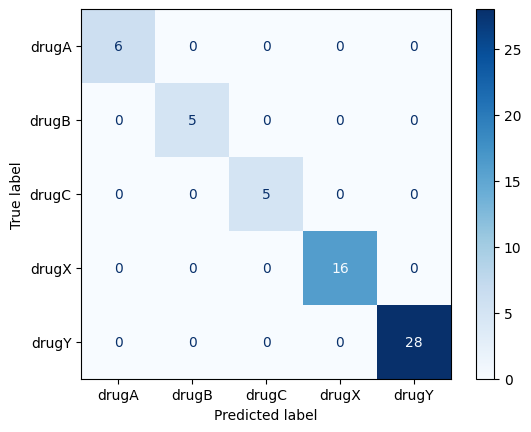
\includegraphics[width=0.4\linewidth]{img/Q3/Basic test.png}
		}
	\caption{Confusion Matrix}
	\label{fig: Q3 best cm}
\end{figure}

در انتها به سراغ 
post-pruning
می‌رویم و با استفاده از کد زیر چند 
$\alpha$
متفاوت را تست می‌کنیم که نتیجه آن در 
\autoref{fig:alpha}
قابل مشاهده است. در نتیجه 
post-pruning 
روی درخت به وجود آمده توست مجموعه داده دارو تاثیر منفی خواهد داشت.
\begin{LTR}
	\begin{lstlisting}[language=Python, caption=best alpha]
clf = DecisionTreeClassifier(random_state=53)
path = clf.cost_complexity_pruning_path(X_train, y_train)
ccp_alphas, impurities = path.ccp_alphas, path.impurities
clfs = []
for ccp_alpha in ccp_alphas:
    clf = DecisionTreeClassifier(random_state=53, ccp_alpha=ccp_alpha)
    clf.fit(X_train, y_train)
    clfs.append(clf)
	\end{lstlisting}
\end{LTR}
\begin{figure}[H]
\centering
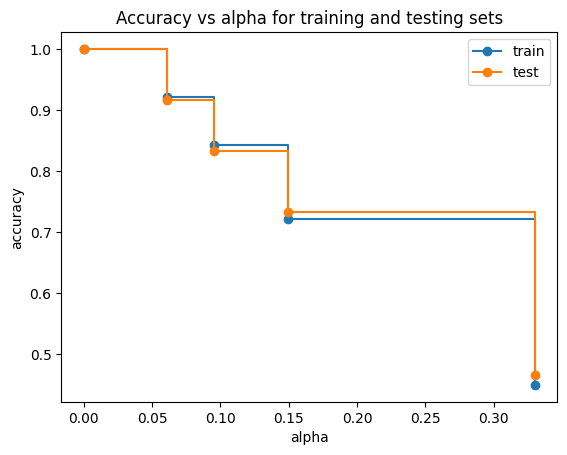
\includegraphics[width=0.7\linewidth]{img/Q3/alpha}
\caption{}
\label{fig:alpha}
\end{figure}


\subsection{بخش سوم}
AdaBoost و RandomForest
 دو تکنیک یادگیری جمعی هستند که می‌توانند عملکرد درخت تصمیم را به طور قابل توجهی بهبود بخشند. این تکنیک‌ها به شرح زیر عمل می‌کنند.
 
{\large \textbf{AdaBoost}:} 
AdaBoost 
یک تکنیک تقویت است که بر بهبود دقت پیش‌بینی‌ها با ترکیب چندین درخت تصمیم تکیه دارد. ایده کلیدی پشت AdaBoost
 تنظیم وزن داده‌های آموزشی بر اساس عملکرد درخت قبلی است. 
 
طی فرایند آموزش یک مدل 
AdaBoost
 ابتدا، وزن‌ تمام نمونه‌ها برابر یکدیگر قرار داده می‌شود. سپس یک درخت تصمیم‌گیری با استفاده از این داده‌هاآموزش داده می‌شود. در ادامه، وزن نمونه‌هایی که نادرست طبقه‌بندی‌شده، افزایش می‌یابد تا درخت بعدی بر روی آن‌ها تمرکز کند. این فرایند برای تعداد مشخصی از تکرارها یا تا رسیدن به دقت مطلوب تکرار می‌شود. مدل نهایی یک جمع وزن‌دار از مجموعه درخت‌‌ها است، که در آن درخت‌های دقیق‌تر وزن بیشتری دارند. فرایند آموزش یک مدل AdaBoost در 
 \autoref{fig:ada}
 آورده شده است.
 
 
\begin{figure}[H]
\centering
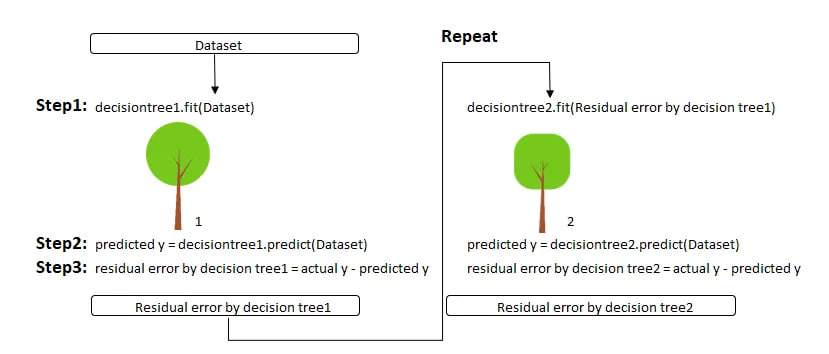
\includegraphics[width=1\linewidth]{img/Q3/ada}
\caption{نحوه عملکرد و آموزش مدل AdaBoost \cite{towardsdatascience2020ensemblelearning}}
\label{fig:ada}
\end{figure}

{\large \textbf{RandomForest}:} 
RandomForest 
یک  است که با یک مجموعه از درختان تصمیم، یک جنگل تصمیم می‌سازد که هر کدام از درختان این جنگل بر روی یک زیرمجموعه تصادفی از داده‌ها و ویژگی‌ها آموزش داده می‌شوند. 

در این روش، ابتدا زیرمجموعه‌های تصادفی از داده‌های آموزشی انتخاب می‌شوند. سپس یک درخت تصمیم‌گیری بر روی هر زیرمجموعه آموزش داده می‌شود. هر درخت به طور مستقل یک پیش‌بینی انجام می‌دهد و پیش‌بینی نهایی با رأی اکثریت بین تمامی درختان انجام می‌شود. این روش مؤثر است زیرا درختان را با آموزش آن‌ها بر روی نمونه‌ها و زیرمجموعه‌های ویژگی‌های مختلف، از هم جدا می‌کند. تجمیع پیش‌بینی‌ها از چندین درخت به طور کلی به عملکرد بهتری نسبت به هر درخت منفرد منجر می‌شود.

هر دو روش AdaBoost و RandomForest عملکرد درخت تصمیم‌گیری را بهبود می‌بخشند. در حالی که AdaBoost بر بهبود متوالی و تنظیم وزن‌ها تمرکز دارد، RandomForest مجموعه‌ای متنوع از درختان را می‌سازد و نتایج آن‌ها را میانگین می‌گیرد. این دو تکنیک می‌توانند مدلی بهتر ایجاد کنند.
\cite{geeksforgeeks2023differences}

حال با استفاده از کد زیر یک مدل
RandomForest
را آموزش می‌دهیم.


\begin{LTR}
\begin{lstlisting}[language=Python, caption=Random Forest Training]
# Define the parameter grid for the Random Forest
param_grid_rf = {
    'n_estimators': [100, 200, 300],
    'max_features': ['auto', 'sqrt'],
    'max_depth': [4, 6, 8, None],
    'min_samples_split': [2, 5, 10],
    'min_samples_leaf': [1, 2, 4],
    'bootstrap': [True, False]
}

# Initialize the Random Forest classifier
rf_clf = RandomForestClassifier(random_state=53)

# Initialize GridSearchCV
grid_search_rf = GridSearchCV(estimator=rf_clf, param_grid=param_grid_rf, cv=5, n_jobs=-1, )

# Fit GridSearchCV
grid_search_rf.fit(X_train, y_train)

\end{lstlisting}
\end{LTR}

نتایج بدست آمده از مدل فوق به شرح زیر می‌باشد که تمام متریک‌ها برابر 1 شده‌اند و از روی ماتریس درهم‌ریختگی 
\autoref{fig: Q3 rf cm}
 مشخص است که تمام نمونه‌ها به درستی تشخیص داده‌شده‌اند.


\begin{LTR}
\begin{verbatim}
training metrics:
Classification Report:
               precision    recall  f1-score   support

       drugA       1.00      1.00      1.00        17
       drugB       1.00      1.00      1.00        11
       drugC       1.00      1.00      1.00        11
       drugX       1.00      1.00      1.00        38
       drugY       1.00      1.00      1.00        63

    accuracy                           1.00       140
   macro avg       1.00      1.00      1.00       140
weighted avg       1.00      1.00      1.00       140

test metrics:

Classification Report:
               precision    recall  f1-score   support

       drugA       1.00      1.00      1.00         6
       drugB       1.00      1.00      1.00         5
       drugC       1.00      1.00      1.00         5
       drugX       1.00      1.00      1.00        16
       drugY       1.00      1.00      1.00        28

    accuracy                           1.00        60
   macro avg       1.00      1.00      1.00        60
weighted avg       1.00      1.00      1.00        60
\end{verbatim}
\end{LTR}

\begin{figure}[H] 
	\centering
	\subfigure[]{
		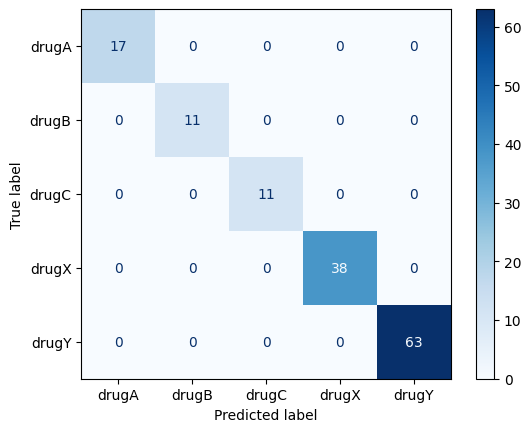
\includegraphics[width=0.4\linewidth]{img/Q3/Basic train.png}
		}
	\subfigure[]{
		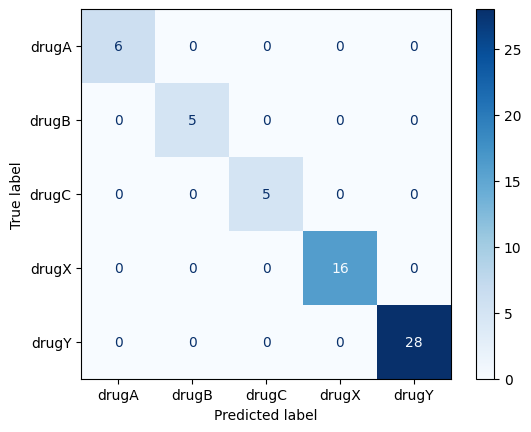
\includegraphics[width=0.4\linewidth]{img/Q3/Basic test.png}
		}
	\caption{Confusion Matrix}
	\label{fig: Q3 rf cm}
\end{figure}


\section{سوال 4}

روش Bayse با تکیه بر توضیح احتمالاتی مسئله و با فرض اینکه رگرسورها از یکدیگر مستقل هستند، از قانون
Bayse 
استفاده می‌کند تا یک مدل طبقه‌بندی را ایجاد کند. با توجه به اینکه الگوریتم به توزیع احتمالاتی وابسته است نرمال کردن دیتاست تاثیری در نتیجه نخواهد داشت بنابراین پیش‌پردازش خاصی لازم نیست. همانطور که در ‎
\autoref{tab:Q4 data}
مشخص است این دیتاست 13 ویژگی را اندازه‌گیری کرده است تا به وسیله آنها پیشبینی انجام شود.

\begin{table}[ht]
\centering
\begin{tabular}{ccccccccccccccc}
\toprule
 & Age & Sex & CP & Trestbps & Chol & FBS & Restecg & Thalach & Exang & Oldpeak & Slope & CA & Thal & Target \\
\midrule
0 & 52 & 1 & 0 & 125 & 212 & 0 & 1 & 168 & 0 & 1.0 & 2 & 2 & 3 & 0 \\
1 & 53 & 1 & 0 & 140 & 203 & 1 & 0 & 155 & 1 & 3.1 & 0 & 0 & 3 & 0 \\
2 & 70 & 1 & 0 & 145 & 174 & 0 & 1 & 125 & 1 & 2.6 & 0 & 0 & 3 & 0 \\
3 & 61 & 1 & 0 & 148 & 203 & 0 & 1 & 161 & 0 & 0.0 & 2 & 1 & 3 & 0 \\
4 & 62 & 0 & 0 & 138 & 294 & 1 & 1 & 106 & 0 & 1.9 & 1 & 3 & 2 & 0 \\
\bottomrule
\end{tabular}
\caption{Sample Data}
\label{tab:sample_data}
\end{table}

در ادامه برای آموزش مدل مبتنی بر
Bayse
مجموعه داده موجود با استفاده از کد زیر به دو قسمت آموزش و ارزیابی تقسیم می‌شود و پس از آن مدل به روی دیتاست مذکور تنظیم می‌شود.

\begin{LTR}
\begin{lstlisting}[language=Python, caption=best alpha]
# Split data into training and testing sets
X_train, X_test, y_train, y_test = train_test_split(X, y, test_size=0.2, random_state=53)

# Initialize and train the Gaussian Naive Bayes classifier
model = GaussianNB()X_train, y_train)

# Train model
model.fit(X_train, y_train)
\end{lstlisting}
\end{LTR}

نتایج بدست آمده از مدل فوق روی مجموعه داده ارزیابی به شرح زیر می‌باشد. با توجه به متریک 
Recall
می‌توانیم به این نتیجه برسیم که مدل در پیدا کردن نمونه‌های کلاس 0، نسبت به نمونه‌های کلاس 1 ضعیف‌تر عمل کرده است و با اینکه تعداد نمونه‌ها در هر دو کلاس یکسان بوده اما دقت مدل در پیدا کردن کلاس 0، 
10\%
ضعیف‌تر بوده اما از سوی دیگر اگر مدل درمورد یک نمونه از کلاس 0 پیشبینی کرده، احتمال اینکه این پیشبینی درست باشد بیشتر است و این مسئله از متریک 
Precision
قابل نتیجه می‌باشد. به صورت کلی دقت مدل در پیدا کردن و میزان درست بودن پیشبینی‌هایش از رابطه‌ای بین 
Precision و Recall 
نتیجه می‌شود که به آن 
f-1 Score
می‌گویند. 
f-1 Score 
برای هردو کلاس بالای 
80\% 
است و اختلاف کمی دارد که نشان می‌دهد مدل علاوه‌براینکه از دقت مناسبی برخوردار است، به کلاس خاصی متمایل نشده است. این نتایج در ماتریس درهم‌ریختگی موجود در 
\autoref{fig: Q4 cm}
قابل ملاحضه است.
\begin{LTR}
\begin{verbatim}
Classification Report:
               precision    recall  f1-score   support

     Class 0       0.86      0.77      0.81       102
     Class 1       0.80      0.87      0.83       103

    accuracy                           0.82       205
   macro avg       0.83      0.82      0.82       205
weighted avg       0.83      0.82      0.82       205
\end{verbatim}
\end{LTR}

\begin{figure}[H] 
	\centering
	\subfigure[]{
		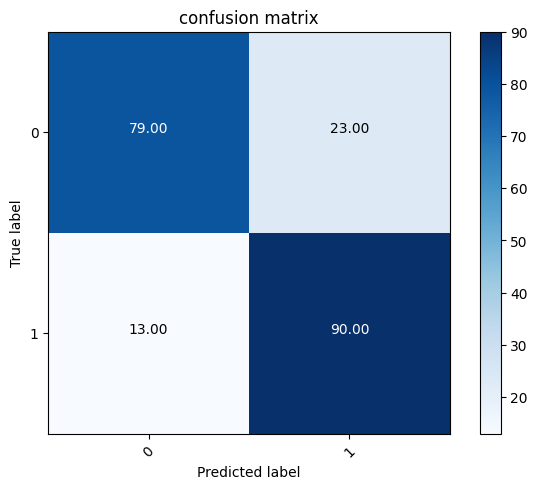
\includegraphics[width=0.4\linewidth]{img/Q4/cm.png}
		}
	\subfigure[]{
		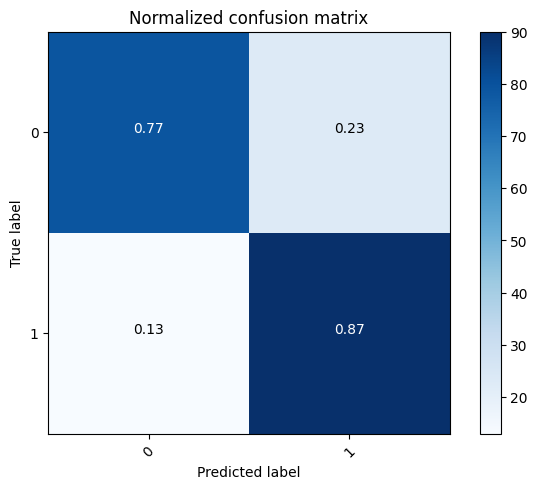
\includegraphics[width=0.4\linewidth]{img/Q4/cmn.png}
		}
	\caption{Confusion Matrix}
	\label{fig: Q4 cm}
\end{figure}

در کتابخانه
 Scikit-learn،
 اصطلاحات 
 micro
  و 
  macro
   به روش‌های مختلف میانگین‌گیری معیارها مانند
   Recall، Precision و  f-1 Score
   در مسائل طبقه‌بندی چاشاره دارند. روش micro متریک‌ها را به صورت کلی در شرایطی هر پیش‌بینی ارزش یکسانی دارد محاسبه می‌کند، به عبارت دیگر این روش تمام 
   true positives، true negative، false negatives و false positives 
   را برای محاسبه متریک موردنظر حساب می‌کند
   که می‌تواند تحت تأثیر 
   imbalance
    بودن کلاس‌ها قرار گیرد اما عملکرد کلی جامعی را ارائه می‌دهد. در مقابل، میانگین‌گیری
    macro
     معیارها را برای هر کلاس به طور مستقل محاسبه و سپس میانگین می‌گیرد، و به هر کلاس بدون توجه به فراوانی آن وزن مساوی می‌دهد، که آن را نسبت به
     imbalance
      کلاس‌ها کمتر حساس می‌کند. انتخاب بین میانگین‌گیری micro و macro بستگی به این دارد که آیا می‌خواهید بر عملکرد کلی تأکید کنید یا عملکرد متعادل در تمام کلاس‌ها مدنظر می‌باشد.

در انتها به ارزیابی مدل روی 5 نمونه از داده‌ها می‌پردازیم. با استفاده از کد زیر 5 نمونه به صورت تصادفی از مجموعه داده استخراج می‌شود و سپس مدل روی این داده پیشبینی انجام می‌دهد و در گام آخر پیشبینی به همراه کلاس واقعی نمایش داده می‌شود که این نتایج در 
\autoref{tab:Q4 t}
قابل مشاهده می‌باشد. این مدل تنها در یک مورد از 5 مورد اشتباه کرده است که کلاس را 1 تشخیص داده اما این درحالی است که کلاس واقعی 0 بوده است.


\begin{LTR}
\begin{verbatim}
test_data = data.sample(n=5, random_state=53)
pred = model.predict(test_data.drop("target", axis='columns'))
test_data['predictions'] = pred
test_data.head()
\end{verbatim}
\end{LTR}

\begin{table}[H]
\centering
\begin{tabular}{cccccccccccccccc}
\toprule
 & Age & Sex & CP & Trestbps & Chol & FBS & Restecg & Thalach & Exang & Oldpeak & Slope & CA & Thal & Target & Predictions \\
\midrule
420 & 57 & 0 & 0 & 128 & 303 & 0 & 0 & 159 & 0 & 0.0 & 2 & 1 & 2 & 1 & 1 \\
706 & 57 & 1 & 2 & 128 & 229 & 0 & 0 & 150 & 0 & 0.4 & 1 & 1 & 3 & 0 & 1 \\
673 & 54 & 1 & 2 & 120 & 258 & 0 & 0 & 147 & 0 & 0.4 & 1 & 0 & 3 & 1 & 1 \\
246 & 54 & 1 & 1 & 192 & 283 & 0 & 0 & 195 & 0 & 0.0 & 2 & 1 & 3 & 0 & 0 \\
187 & 56 & 1 & 0 & 125 & 249 & 1 & 0 & 144 & 1 & 1.2 & 1 & 1 & 2 & 0 & 0 \\
\bottomrule
\end{tabular}
\caption{Test Data}
\label{tab:Q4 t}
\end{table}



\bibliographystyle{plain}
\bibliography{references}
\end{document}

